\documentclass[11pt]{article}
\usepackage[a4paper,margin=1in]{geometry}
\usepackage{graphicx}
\usepackage{booktabs}
\usepackage{float}
\usepackage{siunitx}
\title{Telemetry-Based Analysis of Lando Norris's 2026 Fastest Laps in Japan and Miami}
\author{FastF1 Data Analysis}
\date{\today}

\begin{document}
\maketitle

\section{Introduction}
The 2026 Formula One calendar created an unusual competitive context. After the cancellation of the Bahrain and Saudi Arabian Grands Prix, teams had a four-week spring break in which they could prepare mechanical, aerodynamic, and energy-management updates. This report studies Lando Norris's race fastest laps at the 2026 Japanese and Miami Grands Prix using FastF1 telemetry. Norris finished fifth in Japan but improved to second in Miami, while also winning the Miami Sprint. The central question is whether the public telemetry from his fastest race laps supports the project hypothesis that McLaren's Miami package improved aerodynamic performance and energy deployment, especially on a circuit dominated by long straights and slow-corner exits.

\section{McLaren Upgrade Context}
The project brief identifies four main areas of McLaren development for Miami. First, the aerodynamic package was aimed at increasing downforce for a stop-and-go circuit, where braking stability and traction out of slow corners matter as much as peak speed. Second, the team is described as using a more front-loaded electrical deployment logic, supported by a 350 kW recovery system, to strengthen acceleration immediately after corner exit. Third, lightweight composite components reduced redundant mass and were expected to sharpen transient response. Fourth, suspension geometry and cooling changes were intended to stabilize the platform and improve tyre temperature control. The data analysis below focuses mainly on the first two items because public FastF1 telemetry can provide plausible proxies for aerodynamic balance and acceleration behaviour, while weight, suspension geometry, and cooling performance remain largely hidden from the public data stream.

\section{Method}
The analysis uses FastF1 to load the 2026 race sessions, selects Norris's fastest race lap at each event, and exports car telemetry including speed, distance, throttle, brake, gear, RPM, and DRS state. Because FastF1 does not expose McLaren's internal downforce maps or real ERS deployment power, this report treats aerodynamic and energy-management performance as proxy interpretations. Aerodynamics are evaluated through speed-density structure, the share of high-speed running, and a mid-to-high-speed cornering proxy based on samples between 170 and \SI{270}{km/h} with less than full throttle and no braking. Energy management is evaluated through full-throttle share, DRS use, and speed gain over the first 250 m after low-speed segments. These indicators cannot prove the exact content of McLaren's upgrades, but they can show whether Norris's fastest laps had the shape expected from the stated package.

\begin{table}[H]
\centering
\caption{Summary metrics from Norris's fastest race laps}
\begin{tabular}{lrrrrrrr}
\toprule
Event & Lap time & Mean speed & Top speed & Low-speed & High-speed & Corner proxy & Full throttle \\
 & s & km/h & km/h & share & share & km/h & share \\
\midrule
Japanese Grand Prix & 93.208 & 222.3 & 321.0 & 13.9\% & 37.7\% & 198.7 & 53.6\% \\
Miami Grand Prix & 91.869 & 205.8 & 331.0 & 36.6\% & 38.9\% & 224.6 & 47.2\% \\
\bottomrule
\end{tabular}
\end{table}

\section{Speed Distribution and Track Character}
Figure~\ref{fig:density} compares the speed distribution of the two fastest laps. The Japanese lap is expected to display a larger concentration in the medium and high-speed range because Suzuka is a flowing circuit with long sequences such as the Esses, Degner, Spoon, and 130R. The Miami lap, by contrast, should have a more polarized profile: repeated braking zones and very slow corners lower the left side of the distribution, while the long straights raise the high-speed tail. In the exported metrics, Japan records a low-speed share of 13.9\%, while Miami records 36.6\%, a difference of 22.7 percentage points. The high-speed share changes by 1.3 percentage points from Japan to Miami. This supports the qualitative distinction between Suzuka's sustained-flow character and Miami's stop-and-go demand profile.

\begin{figure}[H]
\centering
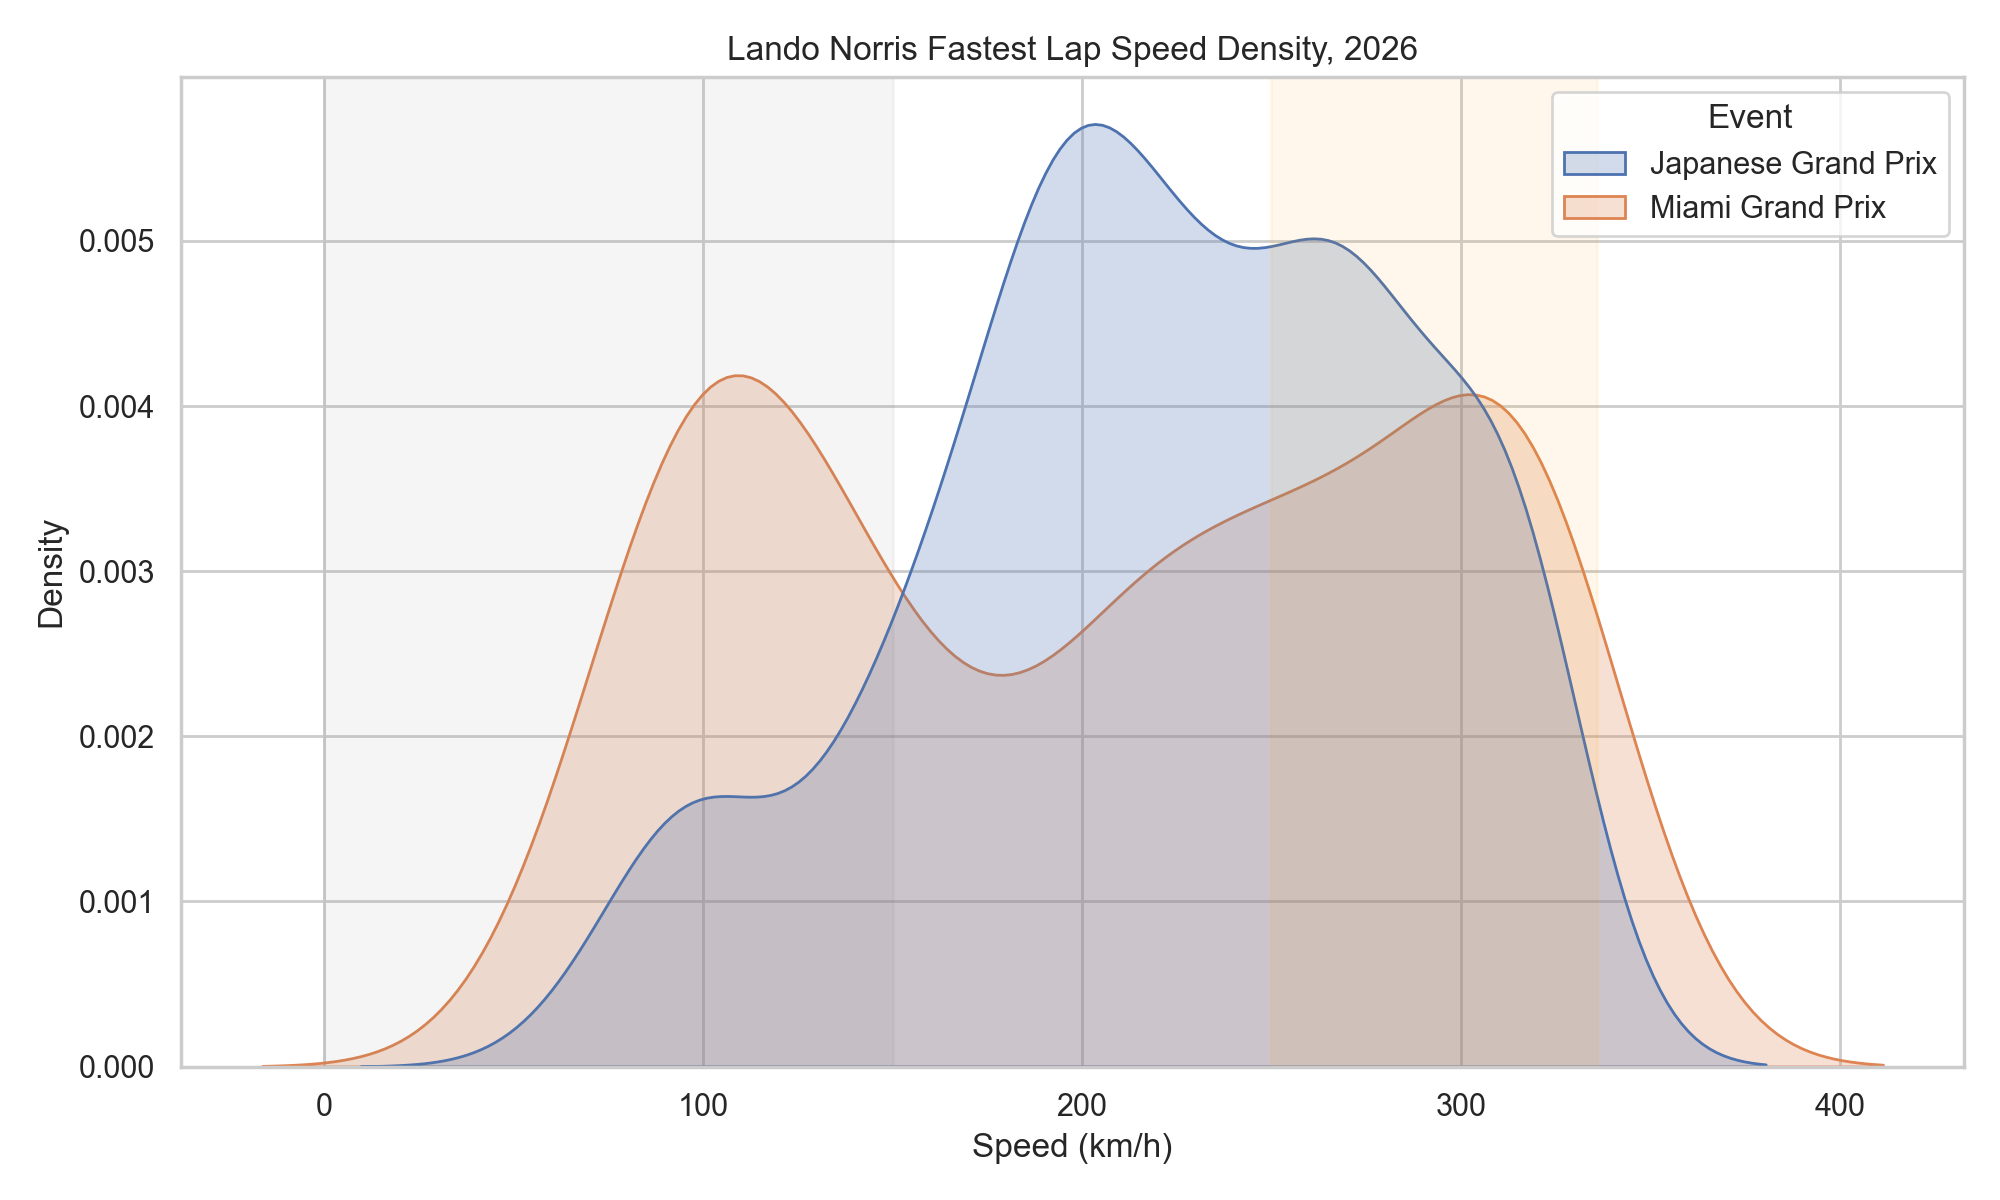
\includegraphics[width=0.92\linewidth]{../figures/norris_speed_density_2026.png}
\caption{Speed density for Norris's fastest race laps in Japan and Miami.}
\label{fig:density}
\end{figure}

\section{Aerodynamic Interpretation}
McLaren's Miami update is described as increasing downforce while preserving responsiveness. The telemetry does not measure downforce directly, but the speed trace in Figure~\ref{fig:speedtrace} gives a useful proxy. A stronger aerodynamic platform should allow the driver to carry speed through medium and high-speed changes of direction without excessive braking or throttle hesitation. The cornering proxy is 198.7 km/h for Japan and 224.6 km/h for Miami. These numbers must be read with circuit context rather than as a simple ranking, because Suzuka and Miami ask very different questions of the car. The Miami evidence is most meaningful when combined with Norris's ability to leave slow zones cleanly and still achieve a top speed of 331.0 km/h. That combination is consistent with an aerodynamic package that added stability and traction-supporting load without creating an excessive straight-line penalty.

\begin{figure}[H]
\centering
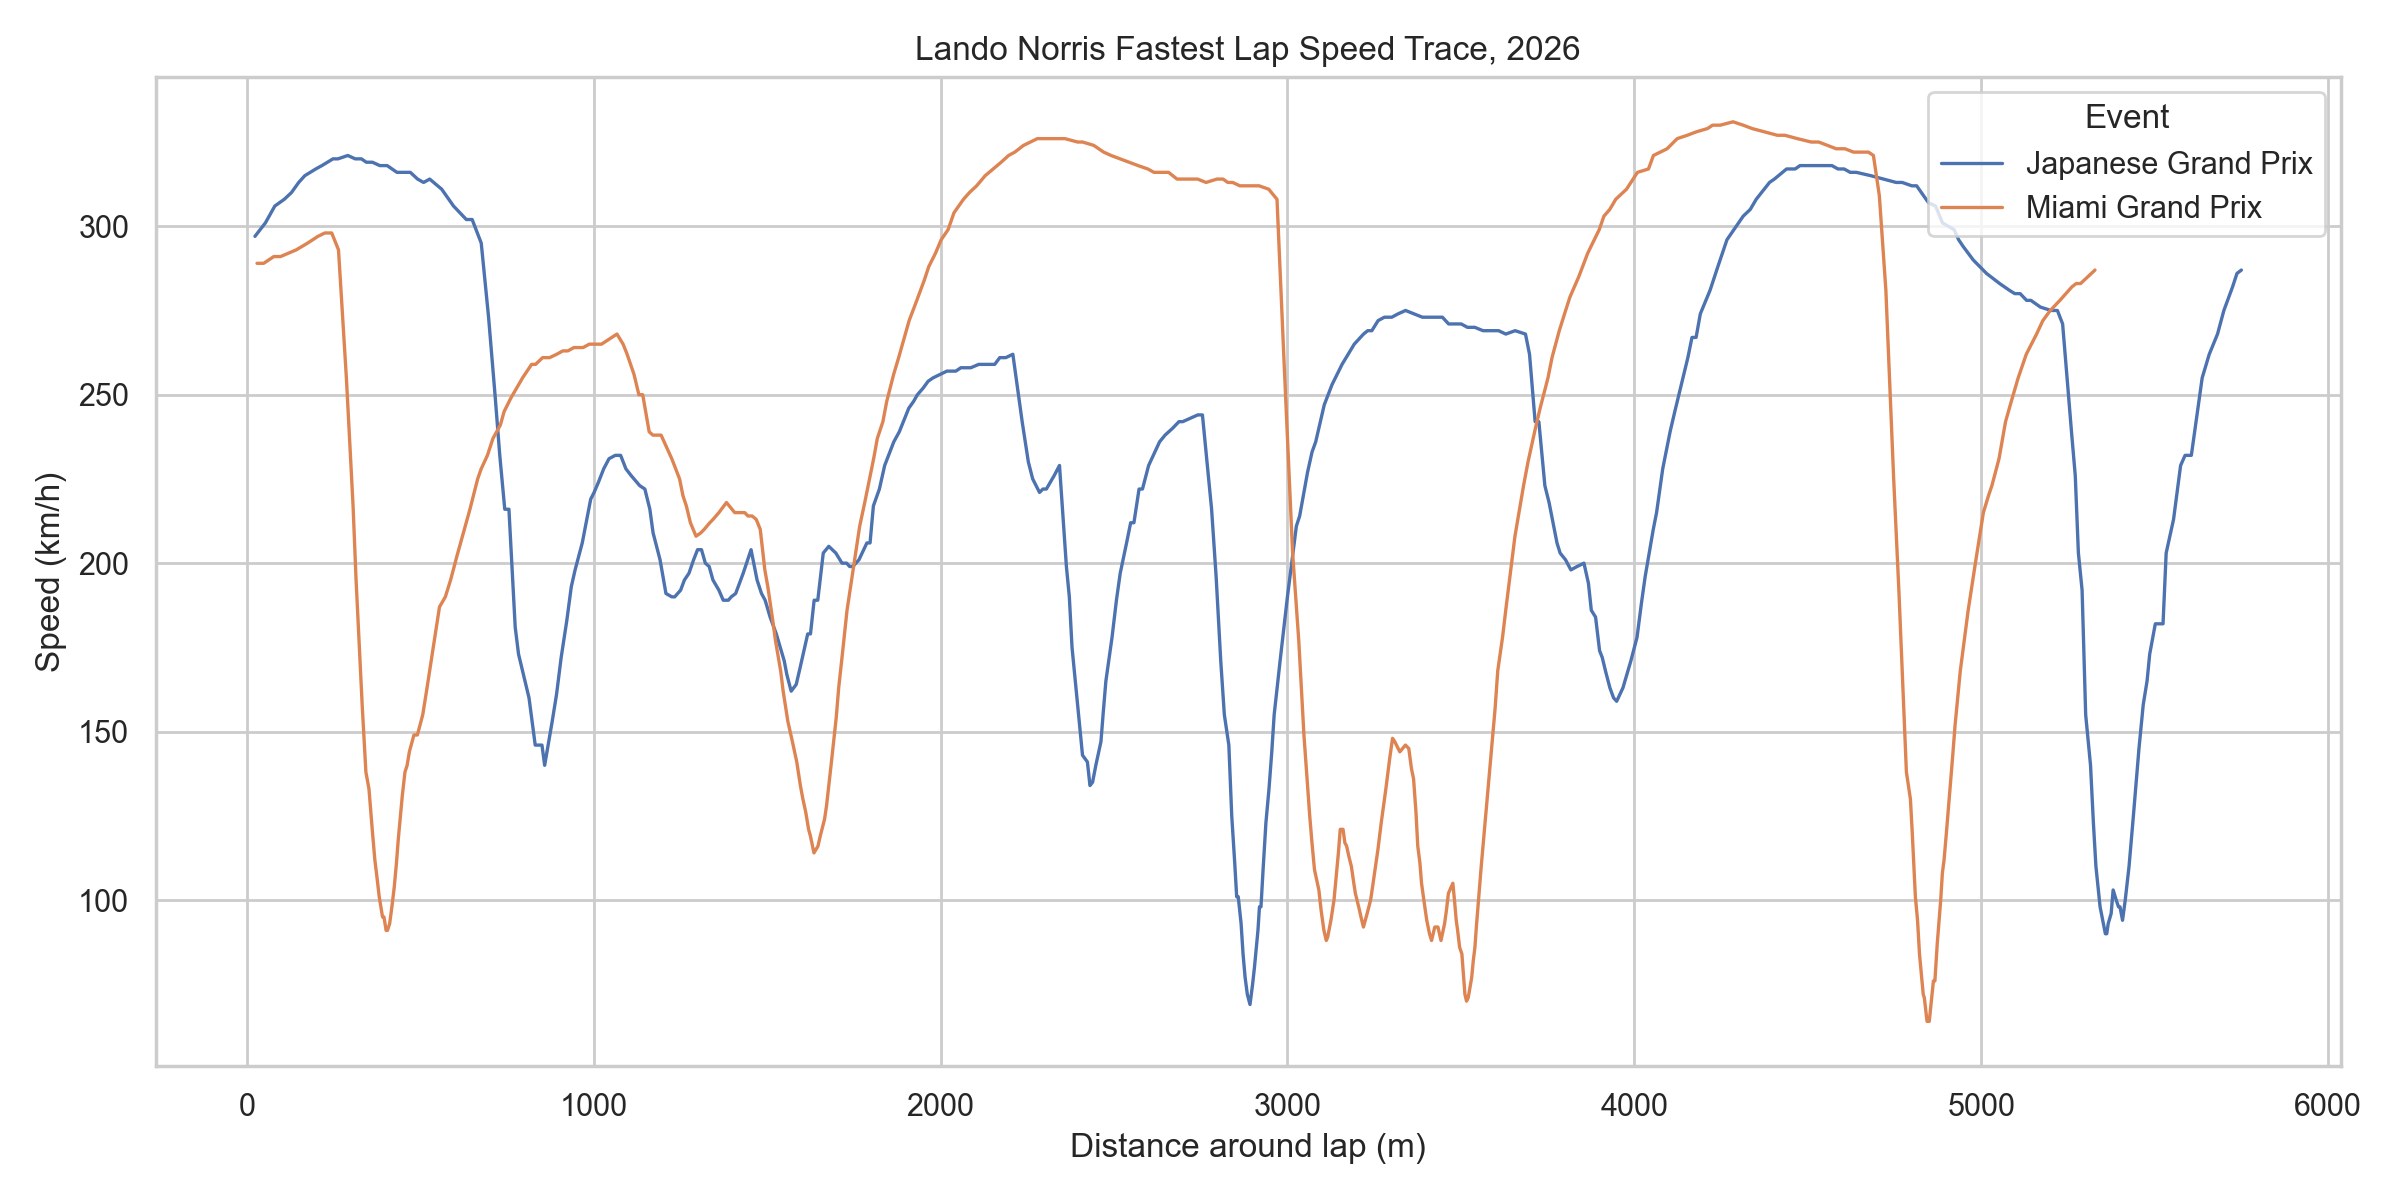
\includegraphics[width=0.92\linewidth]{../figures/norris_speed_distance_2026.png}
\caption{Speed trace by lap distance. The different shapes reveal Suzuka's flowing sections and Miami's repeated stop-and-go phases.}
\label{fig:speedtrace}
\end{figure}

\section{Energy-Management Interpretation}
The project brief states that McLaren introduced a more front-loaded electrical deployment strategy in Miami. Since the public feed does not include ERS power, the best available proxy is the quality of acceleration after low-speed corners. Figure~\ref{fig:exitgain} compares the speed gained in the first 250 m after the slowest segments detected on each lap. Miami's layout makes this indicator especially relevant because lap time is strongly affected by how early the car can deploy torque after tight corners and then sustain acceleration onto the straights. Norris's full-throttle share is 53.6\% in Japan and 47.2\% in Miami, a change of -6.4 percentage points, but Miami's lower full-throttle share is partly a circuit-layout effect caused by more braking and rotation phases. The clearer acceleration proxy is exit speed gain: the detected low-speed exits average 89.7 km/h over 250 m in Japan and 107.2 km/h in Miami, with Miami reaching a maximum gain of 121.0 km/h. This supports the claim that the car was able to convert slow-corner exits into rapid speed build-up, which is the strongest public-telemetry signature of the claimed energy-management change.

\begin{figure}[H]
\centering
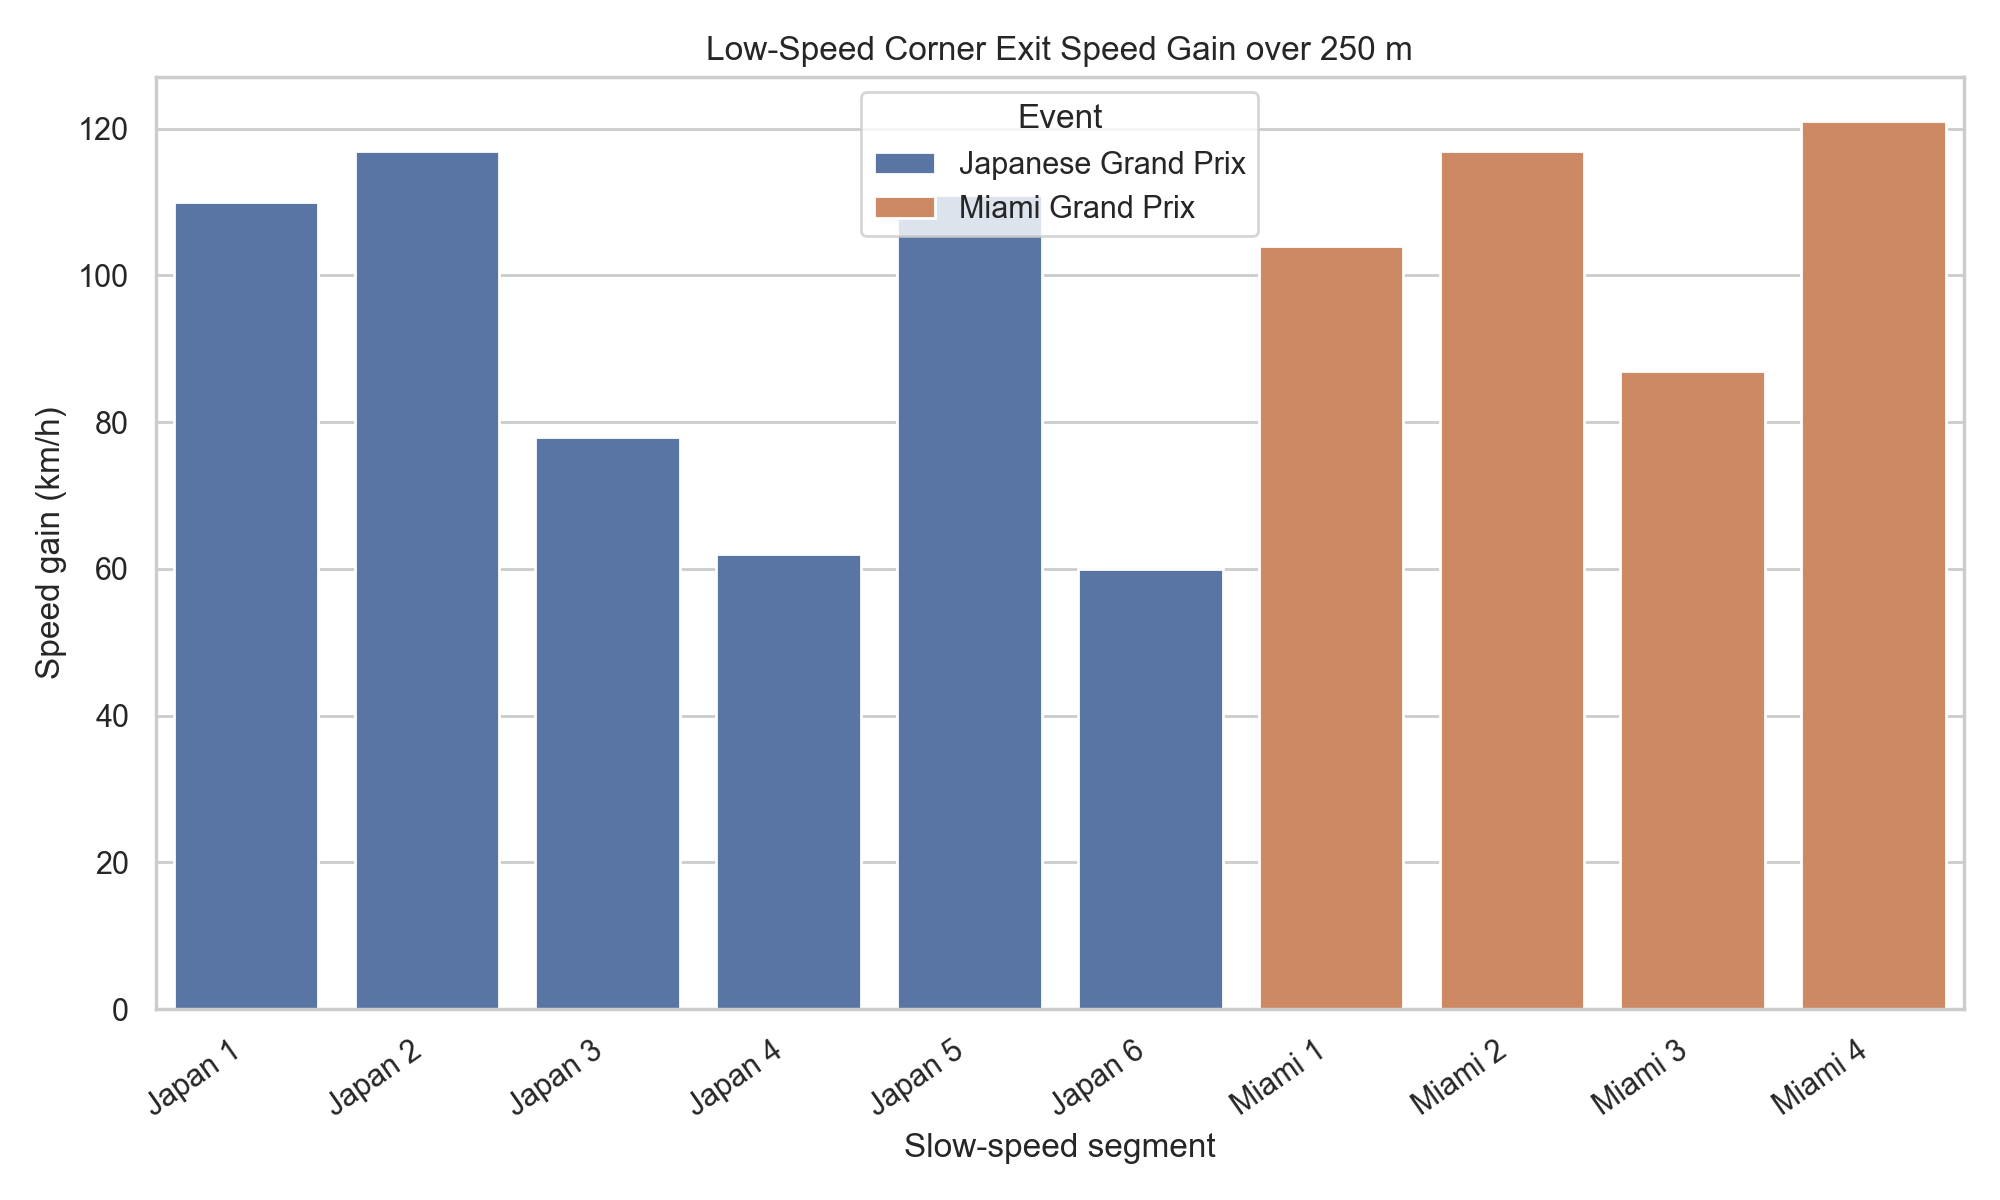
\includegraphics[width=0.92\linewidth]{../figures/norris_exit_gain_2026.png}
\caption{Speed gain over 250 m after detected low-speed segments. This acts as a public-data proxy for corner-exit deployment and traction.}
\label{fig:exitgain}
\end{figure}

\section{Conclusion}
The FastF1 fastest-lap comparison supports the broader conclusion that McLaren's upgrade package was effective in Miami, while also showing the limits of what public telemetry can prove. Japan and Miami impose different demands: Suzuka rewards aerodynamic efficiency and sustained balance through medium and high-speed corners, whereas Miami rewards braking stability, traction, and powerful exits onto long straights. Norris's Miami performance, including his Sprint victory and the team's double podium in the Grand Prix, is consistent with a package that improved the car's stop-and-go performance without sacrificing competitive top-end speed. The speed density, speed trace, and low-speed exit metrics provide data support for the argument that the aerodynamic and energy-management changes worked together. The evidence is therefore strongest when framed as telemetry-backed interpretation rather than direct measurement of McLaren's internal upgrade values.

\end{document}
